%% ----------------------------------------------------------------
%% Background.tex
%% ----------------------------------------------------------------
\chapter{Background and report of literature search}

There were lots of different algorithms existing for object detection and tracking. Some of those algorithms were investigated in this project in order to identify a set of suitable algorithms that were both accurate and efficient enough to analysis video stream from camera in real-time.

\section{Background subtraction}

Being able to detect objects in a video frame is the first, also the most difficult and important step to do object tracking. This is generally accomplished by separation of foreground objects and background image. Three different object detection methodologies were investigated in this project.

\subsection{Colour based}
\label{bgs:colour}

Colour can provides enough information of a specific object. For easier analysis of colour information, a hue-saturation-value (HSV) colourspace \cite[p.~301]{colourspace} representation converted from the original RGB colourspace is usually used, because it would be easier to filter a range of colour based on hue, saturation and brightness.

A simple colour based foreground mask can be generated easily by filtering target colour. For example, an simple implementation \cite{MOTBOC.git} based on colour filtering object detection, as shown in \fref{Figure:MOTBOC}.

\begin{figure}[H]
  \centering
  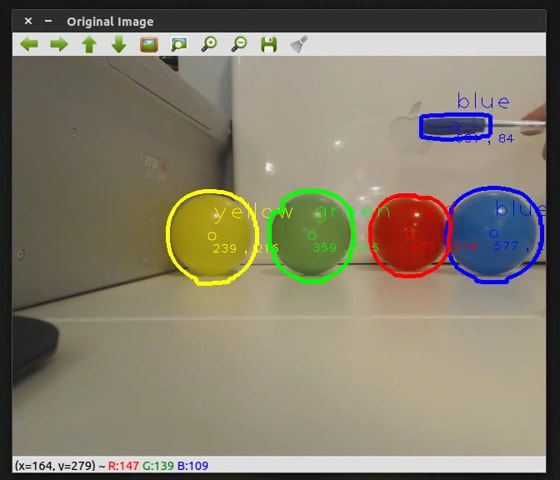
\includegraphics[width=0.6\columnwidth]{MOTBOC}
  \caption{Multi Object Tracking Based on Color (adapted from \cite{MOTBOC.git})}
  \label{Figure:MOTBOC}
\end{figure}

This implementation doesn't require a lot of computation, thus was very fast, could be suitable for robots that are tracking sonething like a single coloured ball or piece of paper, also could be useful for line racing car projects.

\subsection{Shape based}

Another important information about an object is its shape. By extracting hard object edges in the scene than apply appropriate shape transformation and filtering algorithms, an object could also be detected based on the shape.

\fref{Figure:circles} shows the image processed by circle detection, based on OpenCV's implementation of Hough Circle Transform \cite{opencv:hough_circle}. The frame captured from camera (\fref{Figure:edges:original}), was converted to gray scale and blurred first, as shown in \fref{Figure:edges:blur}. Smooth was necessarily to reduce possibly false circles that may be detected. Afterwards the object edges in the image was extracted as in \fref{Figure:edges:edges}. Finally \fref{Figure:edges:circles} shows the circles detected by the algorithm.

\begin{figure}[H]
  \centering
  \subfigure [] {
    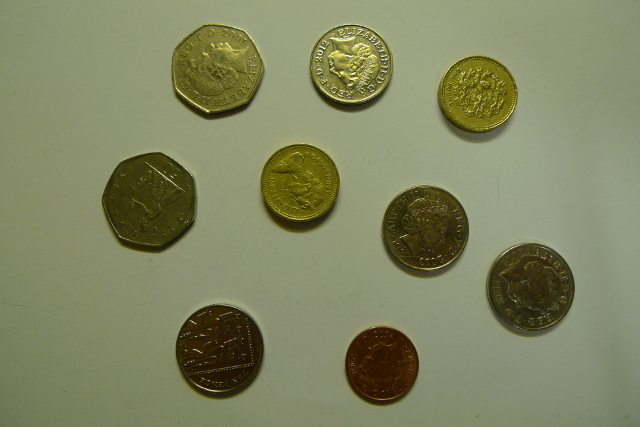
\includegraphics[width=0.45\columnwidth]{simple_original}
    \label{Figure:edges:original}
  }
  \subfigure [] {
    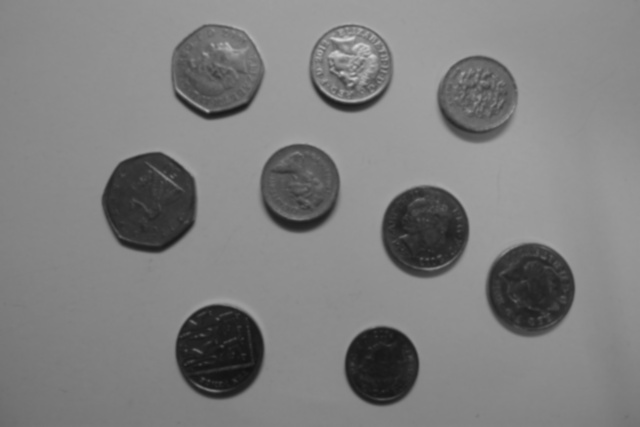
\includegraphics[width=0.45\columnwidth]{simple_blur}
    \label{Figure:edges:blur}
  }
  \subfigure [] {
    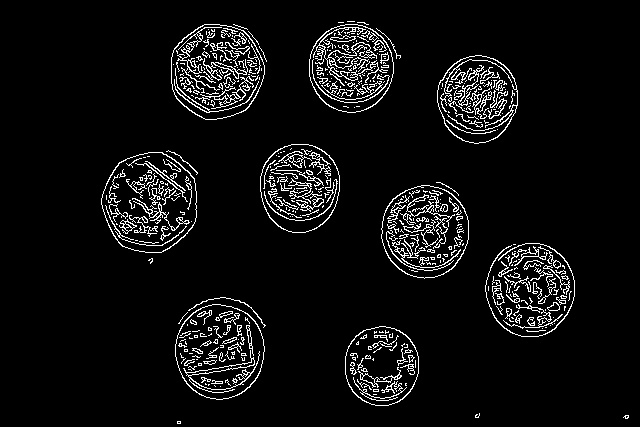
\includegraphics[width=0.45\columnwidth]{simple_edges}
    \label{Figure:edges:edges}
  }
  \subfigure [] {
    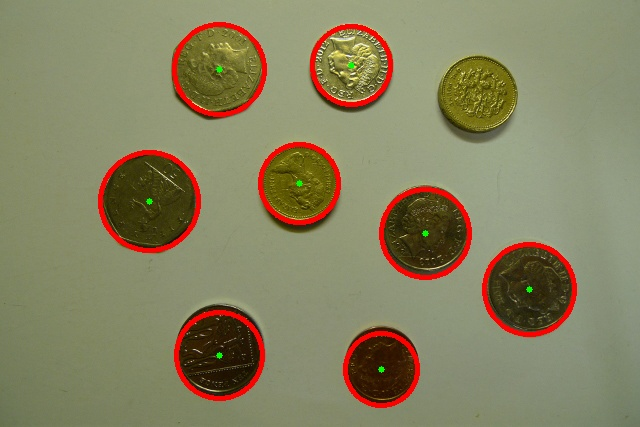
\includegraphics[width=0.45\columnwidth]{simple_circles}
    \label{Figure:edges:circles}
  }
  \caption{Circle detection. \subref{Figure:edges:original} The original image, \subref{Figure:edges:blur} image converted to gray scale and blurred, \subref{Figure:edges:edges} edges detected, \subref{Figure:edges:circles} circles detected}
  \label{Figure:circles}
\end{figure}

This implementation could be suitable for ball tracking purpose. By combining with the simple colour filtering algorithm as described in Section \ref{bgs:colour}, a single coloured ball could be efficiently tracked.

\subsection{Cascade Classifier}

Cascade classifier \cite{cascade} is another widely used technique for object detection. It concatenates several classifiers detecting different object features to recognise objects, and it can be trained both positively and negatively to improve accuracy. It was usually used for object classify, for example recognise human and different classes of vehicles in a single frame.

The OpenCV's cascade classifier implementation \cite{opencv:cc} of face and eye detection was investigated as shown in \fref{Figure:cc_face}.

\begin{figure}[H]
  \centering
  \includegraphics[width=0.6\columnwidth]{"CC face"}
  \caption{Face and eye detection cascade classifiers, detected face was circled by pink, whereas detected eyes were circled by blue}
  \label{Figure:cc_face}
\end{figure}

\subsection{Motion based}

By differenceing current frame and previous frames then probably build up a background model image, it is also possible to detects moving objects efficiently. The BGSLibrary \cite{bgslibrary} is specifically developed for this purpose, it offers 37 different background substraction algorithms using OpenCV, published under GNU GPL v3 license.

This type of algorithms suit well for static camera movement tracking, therefore was used in this project.

\section{Movement tracking}

After obtained the foreground object mask, they need to be interpreted as objects, then the object can be detected and tracked based on its position.

\subsection{Connected component analysis} \label{blob}

Connected component analysis, or Connected component labeling, is used for detecting connected regions (blobs). A blob detector can be used to mark and labeling individual objects from the foreground mask, therefore obtain parameters such as size, position and orientation of the object. Afterwards, by comparing nearby objects from previous frames, the objects can be tracked, and movement parameter such as velocity and acceleration can then be obtained by physical modelling.

There were also lots of free and open source blob detection libraries available, e.g. the simple blob detector came with OpenCV \cite{opencv:blob}, cvBlob library \cite{cvblob}.

\subsection{Continuously Adaptive Meanshift}

Continuously Adaptive Meanshift (CAMshift) \cite{bradski1998computer} is a technique used to track a region of interest (ROI) in continuous frame sequences. It is based on Meanshift algorithm, which only track a fixed size ROI window, whereas CAMshift can handle target resize and rotation. In order to determine the ROI for CAMshift, the blob detector as described in Section \ref{blob} can also be used. This algorithm can also be easily implemented using OpenCV \cite{opencv:camshift}, and was used by lots of researches such as \cite{chu2007object}, \cite{xu2012moving} and \cite{nouar2006improved}.
